\documentclass[12pt,]{book}
\usepackage[utf8]{inputenc}
\usepackage[T1]{fontenc}
\usepackage{mathptmx}
\usepackage{geometry}
\usepackage{mathtools}
\usepackage[english]{babel}
\usepackage{graphicx}
\usepackage[os=win]{menukeys}
\usepackage[figurename=Gambar]{caption}
\usepackage{hyperref}
\usepackage{minted}
\usepackage{float}
\usepackage{pdflscape}
\usepackage{pdfpages}
\usepackage {tikz}

\addto\captionsenglish{\renewcommand{\contentsname}{Daftar Isi}}
\addto\captionsenglish{\renewcommand{\bibname}{Referensi}}

\hypersetup{
	colorlinks=true, %set true if you want colored links
	linktoc=all,     %set to all if you want both sections and subsections linked
	linkcolor=blue,  %choose some color if you want links to stand out
}

\geometry{
	a4paper,
	left=15mm,
	right=10mm,
	top=10mm,
	bottom=10mm,
}

\tikzstyle{squared} = [rectangle, rounded corners, minimum width=2cm, minimum height=1cm,text centered, draw=black]
\tikzstyle{connect} = [ultra thick,<->]

\title{\Large \bf
	Pengenalan GNU/Linux dan Lingkungan Pemrogramannya.
}

\author{Achmadi ST s.MT}
\date{}

\begin{document}
	\maketitle
	\thispagestyle{empty}
	\pagestyle{empty}
	
	\newpage
	\tableofcontents
	
	\newpage
	\section{GNU/Linux}
	
	\subsection{Pengenalan}
	\hspace{10pt} Linux adalah \textit{kernel} sistem operasi komputer yang dibuat di tahun 1991 oleh mahasiswa Finlandia, Linux Torvald.
	Linux dirancang sangat mirip dengan kernel sistem operasi UNIX yang dibuat oleh lab AT\&T (semacam Telkom di USA).
	Selain Linux, kernel lain yang juga berbasis UNIX antara lain Darwin (MacOS) dan BSD (Berkeley OS).
	
	Kernel adalah bagian terpenting dari sistem operasi.
	Kernel memiliki tugas antara lain:
	\begin{itemize}
		\item Mengatur alokasi memori (RAM) dan processor ()CPU)
		\item Mengatur permintaan layanan/sumber daya hardware dan software
	\end{itemize}
	
	Untuk membentuk sistem operasi yang bisa dipakai, kernel saja tidak cukup.
	Dibutuhkan sistem antar-muka (\textit{interface}) dan software alat bantu (\textit{tools}).
	Disinilah peran GNU. 
	GNU adalah organisasi yang dibentuk oleh Richard Stallman.
	Karya GNU antara lain software interface/tools, translasi, dan dokumentasi.
	Dan karya terbesar GNU adalah membuat lisensi \textit{open-sources} memiliki kekuatan hukum.
	
	Open-source adalah bentuk/model pengembangan software dimana pengembang memberikan hak akses kode sumber (\textit{source-code}) kepada pengguna.
	Open-source memberikan hak kepada pengguna antara lain:
	\begin{itemize}
		\item Hak untuk menggandakan
		\item Hak untuk mempelajari
		\item Hak untuk memodifikasi
		\item Hak untuk menyebarluaskan
	\end{itemize}
	Dalam proses memberikan akses kode sumber, pengembang dapat memberikan hak akses secara berbayar atau bisa juga gratis.
	
	\subsection{Struktur}
	Secara sederhana, struktur sistem operasi GNU/Linux adalah sebagai berikut:
	\begin{center}
		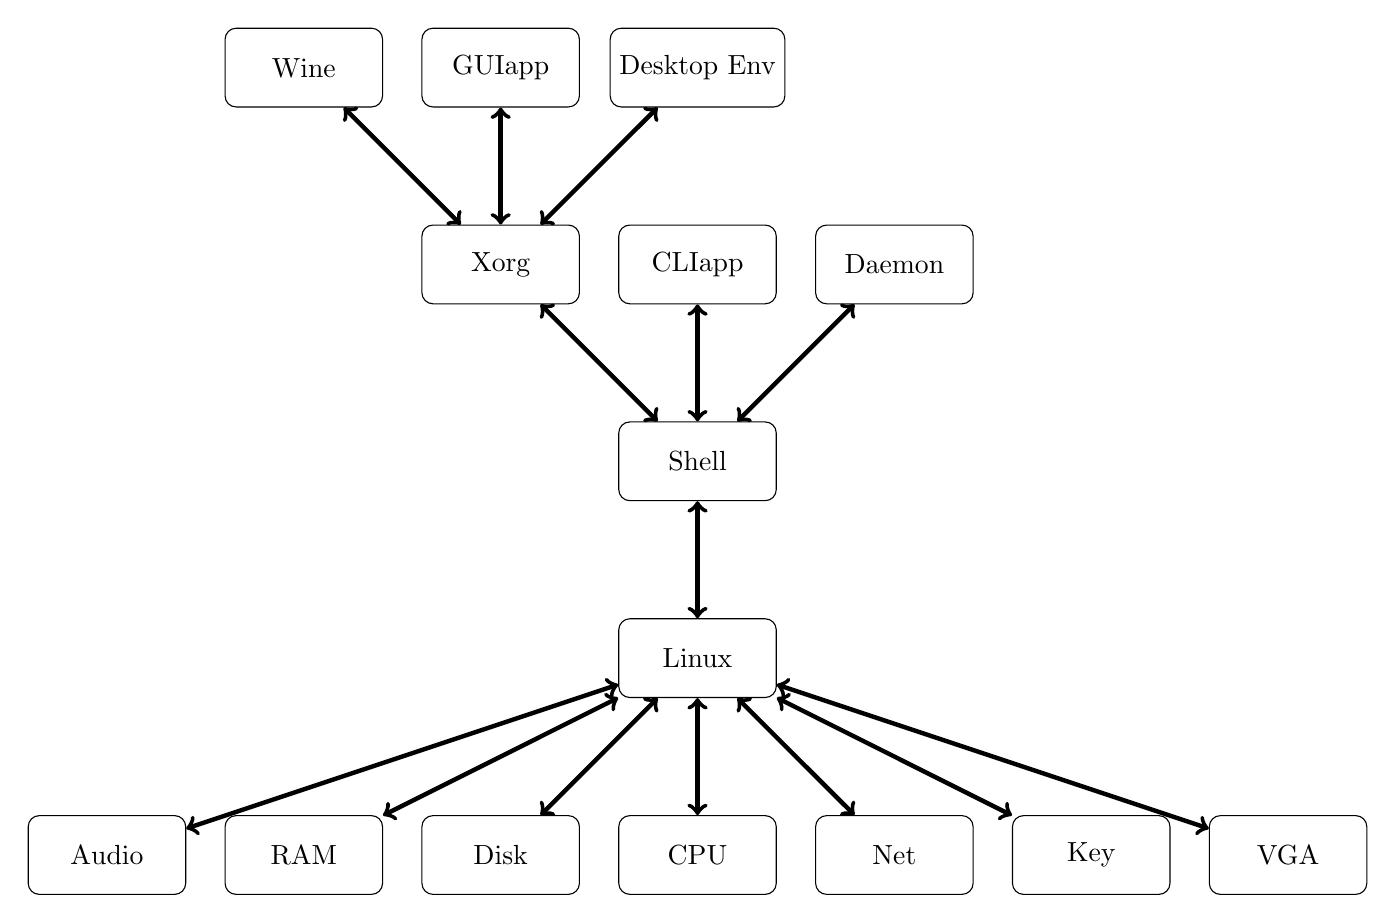
\begin{tikzpicture}[node distance=2.5cm]
		\node (linux) [squared] {Linux};
		\node (shell) [squared, above of=linux] {Shell};
		\node (cpu) [squared, below of=linux] {CPU};
		\node (ram) [squared, left of=cpu] {Disk};
		\node (disk) [squared, left of=ram] {RAM};
		\node (audio) [squared, left of=disk] {Audio};
		\node (net) [squared, right of=cpu] {Net};
		\node (key) [squared, right of=net] {Key};
		\node (vga) [squared, right of=key] {VGA};
		\node (cli) [squared, above of=shell] {CLIapp};
		\node (xorg) [squared, left of=cli] {Xorg};
		\node (gui) [squared, above of=xorg] {GUIapp};
		\node (de) [squared, right of=gui] {Desktop Env};
		\node (daemon) [squared, right of=cli] {Daemon};
		\node (wine) [squared, left of=gui] {Wine};
		
		\draw [connect] (linux) -- (shell);
		\draw [connect] (linux) -- (cpu);
		\draw [connect] (linux) -- (ram);
		\draw [connect] (linux) -- (disk);
		\draw [connect] (linux) -- (audio);
		\draw [connect] (linux) -- (net);
		\draw [connect] (linux) -- (key);
		\draw [connect] (linux) -- (vga);
		\draw [connect] (shell) -- (cli);
		\draw [connect] (shell) -- (xorg);
		\draw [connect] (shell) -- (daemon);
		\draw [connect] (xorg) -- (gui);
		\draw [connect] (xorg) -- (de);
		\draw [connect] (xorg) -- (wine);
		\end{tikzpicture}
	\end{center}

	\subsection{Persiapan VBox}
	
%	\subsection{Instalasi}
%	\subsection{Shell}
%	\subsection{Directory}
%	
%	\section{Pengelola Paket}
%	\subsection{Pengenalan}
%	\subsection{pacman}
%	\subsubsection{install}
%	\subsubsection{remove}
%	\subsubsection{info: available}
%	\subsubsection{info: installed}
%	\subsubsection{non-repo}
%	\subsubsection{update}
%	\subsection{makepkg}
%	\subsection{alternatif}
%	
%	\section{GUI}
%	\subsection{Pengenalan}
%	\subsection{Instalasi}
%	
%	\section{Pemrograman Script Bash}
%	
%	\section{Pemrograman C/C++}
%	
%	\section{Git}
%	
%	\section{Wine/Winemaker}
%	
%	\section{Server HTTP/SSH}
\end{document}